\documentclass[letterpaper,10pt,conference]{ieeeconf}
\IEEEoverridecommandlockouts
\overrideIEEEmargins
\usepackage{amsmath,amssymb,booktabs,cite}
\usepackage[T1]{fontenc}
\usepackage{mathptmx,graphicx,microtype,url}
\usepackage[dvipsnames]{xcolor}
\usepackage{tikz}
\usetikzlibrary{arrows.meta,fit,positioning}
% Explicit evidence placeholders; IDs map to FINAL_TESTS.md.
\newcommand{\missing}[2]{\textcolor{BrickRed}{\textbf{[#1: #2]}}}
\newcommand{\model}{YOLO11-DLA-n}
\title{\LARGE\bf YOLO11-DLA: Adapting YOLO11 for Fallback-Free\\
Object Detection on the NVIDIA Deep Learning Accelerator}
\author{Anonymous Authors}
\begin{document}
\special{pdf:minorversion 4}
\maketitle
\thispagestyle{empty}
\pagestyle{empty}
\begin{abstract}
Embedded robots increasingly share a GPU between perception and other workloads,
but exporting a detector to a dedicated accelerator does not guarantee that its
learned computation leaves the GPU. We present YOLO11-DLA, an adaptation of
YOLO11 that targets fallback-free inference on NVIDIA's Deep Learning
Accelerator (DLA). Two localized changes retain the detector's backbone and
neck structure: a channel-softmax and depthwise-convolution block replaces
spatial self-attention, and a static multi-scale prediction interface places
box decoding and non-maximum suppression outside the compiled graph. On a
Jetson Orin with TensorRT 10.3, the nano model compiles into one DLA loadable
with no GPU-assigned learned layer; unmodified YOLO11n fails strict
compilation. At FP16, batch one, and $640\times640$, median
engine-plus-transfer latency is 27.515\,ms, compared with 34.678\,ms for
unmodified YOLO11n using DLA with GPU fallback, a 20.7\% reduction.
The adapted model remains substantially slower than its own GPU engine
(3.500\,ms). Its retained 500-epoch training record reports 37.581 COCO
AP, while serialized-engine accuracy remains
\missing{P3}{to be measured}. We distinguish compiler placement, engine
timing, and application timing, and identify the remaining accuracy,
concurrent-workload, and energy tests required to assess this design as a
robotic perception component.
\end{abstract}
\section{Introduction}
\label{sec:introduction}
Object detection on an embedded robot operates within a shared compute budget.
The same GPU may execute detection, mapping, learned navigation, and manipulation
policies. NVIDIA Jetson platforms that include a Deep Learning Accelerator
(DLA) offer another execution resource for convolutional networks. Moving a
detector's learned computation to this accelerator is therefore a useful design
option, even when the GPU provides lower isolated latency. Whether that option
improves a robot's behavior depends on the resulting accuracy, application
latency, and interference with concurrent workloads.

A deployment option must first be executable. TensorRT can request DLA
placement while allowing unsupported regions to execute on the GPU
\cite{nvidia_dla_working}. Such a build can run successfully without providing
complete offloading. Supported operator names alone are insufficient: tensor
shapes, normalization axes, precision, and physical I/O layouts also constrain
placement. A detector that is efficient on a GPU may consequently become a
sequence of DLA subgraphs and GPU kernels, with additional layout conversion
between them.

YOLO11 \cite{jocher2024yolo11} illustrates this difficulty. Its convolutional
backbone and neck coexist with spatial self-attention and a decoded prediction
interface. The attention forms matrix products that DLA rejects, while the
usual head flattens feature maps and decodes boxes through an interface that
also prevents strict compilation. Merely enabling GPU fallback leaves both
sources of incompatibility in the deployed system.

We present \emph{YOLO11-DLA}, a localized adaptation that preserves the
surrounding YOLO11 architecture and its distributional detection head. We
replace the terminal C2PSA attention block with C2DLA, which combines
input-dependent channel normalization with local convolution. We also replace
the exported head interface with three raw, static, four-dimensional prediction
maps. Box decoding, confidence filtering, and non-maximum suppression (NMS)
then execute on the host. The evaluated nano instance is denoted \model;
DLA throughout means NVIDIA's accelerator.

Our scope is complete placement of the \emph{learned graph} on one DLA core.
It does not include image preprocessing or variable-cardinality detection
post-processing, and it does not imply that CUDA services, transfers, or shared
DRAM disappear. This distinction is essential when interpreting the robotics
motivation: eliminating GPU-assigned learned layers is a verifiable property,
whereas recovering GPU capacity for another task is a system-level hypothesis.

The contribution is threefold. First, we give an implemented YOLO11 adaptation
with explicit equations, tensor interfaces, and a compiler-based acceptance
criterion. Second, we characterize strict FP16 execution against both a GPU
control and stock YOLO11n with DLA fallback, using build records, engine
inspection, timing traces, and layer profiles. Third, we connect that deployment
boundary to its host-side costs and specify the outstanding tests needed to
establish numerical correctness and utility under a robotic workload.

The current evidence establishes compatibility and its measured latency tradeoff.
The adapted graph compiles as one DLA loadable, whereas stock YOLO11n fails
strict compilation. Its median engine-plus-transfer latency is 20.7\% lower
than the stock fallback configuration, but 7.86 times its own GPU latency.
Neither energy savings nor improved concurrent-task performance are assumed
from that placement result. Missing measurements appear as numbered
placeholders so that the completed study can replace them directly.

\section{Related Work}
\label{sec:related}
\paragraph*{Efficient object detection}
YOLO introduced single-network dense detection \cite{redmon2016yolo}.
Subsequent detectors refine feature extraction, training, and inference:
YOLOv7 emphasizes trainable improvements \cite{wang2023yolov7}, and YOLOv10
studies end-to-end detection without conventional NMS \cite{wang2024yolov10}.
YOLO-ReT targets real-time detection on edge GPUs
\cite{ganesh2022yoloret}. Our reference is the Ultralytics YOLO11 software
implementation \cite{jocher2024yolo11}, with its C3k2 stages, C2PSA block,
multi-scale neck, and distributional box regression. We retain that regression
representation, following the distributed bounding-box formulation associated
with generalized focal loss \cite{li2020gfl}. The target is DLA-compatible
execution of an existing detector family; the evidence here does not establish
a new accuracy--speed frontier across detector families.

YOLOBench evaluates YOLO variants under controlled training and across embedded
hardware \cite{lazarevich2023yolobench}. ActNAS studies activation selection
for efficient YOLO deployment, including the interaction of ReLU/SiLU choices
with target hardware and compiler optimizations \cite{sah2025actnas}.
These comparisons are directly relevant to the retained SiLU operations in
YOLO11-DLA: an activation's cost and support must be assessed on its compiled
representation. We preserve SiLU and verify the resulting sigmoid/product
decomposition on the target, while modifying attention and the output boundary.
The distinction is architectural and experimental; deployment on a neural
accelerator alone is not a new contribution.

\paragraph*{Hardware-aware neural networks}
MnasNet and ProxylessNAS incorporate target-device latency into architecture
selection \cite{tan2019mnasnet,cai2019proxyless}. Once-for-All supports
specialization under multiple deployment constraints \cite{cai2020ofa}, and
MCUNet jointly considers the network and runtime for constrained devices
\cite{lin2020mcunet}. These works motivate measuring the deployed system
instead of relying only on operation counts. Our approach uses a manually
specified adaptation of YOLO11, with strict compilation as a feasibility gate.
We do not perform architecture search or prove that two substitutions are a
minimum over all possible executable designs.

\paragraph*{Attention and compatible operators}
External attention replaces pairwise self-attention with learned projections
through an external memory \cite{guo2023external}. C2DLA is related through its
projection--normalization--projection structure, but uses softmax only along
the channel axis at each spatial position. It does not reproduce external
attention's complete normalization scheme or aggregate distant image positions.
Its spatial interaction comes from a local depthwise convolution and the
inherited backbone. We therefore describe the implemented operation as a
channel-softmax mixer rather than an equivalent form of spatial attention.

\paragraph*{Compilation and heterogeneous deployment}
Graph compilers such as TVM fuse and lower neural operators for target hardware
\cite{chen2018tvm}. TensorRT provides DLA compilation, optional GPU fallback,
and native tensor formats, subject to documented layer restrictions
\cite{nvidia_dla_working}. Compiler transformations can resolve some
source-level incompatibilities, so exported operator counts are explanatory
rather than a sufficient placement test. Our acceptance criterion combines a
fallback-disabled build with inspection of the optimized engine. This places
model structure, exported interface, and compiled placement in the same
experimental comparison.

\section{YOLO11-DLA}
\label{sec:method}
\begin{figure}[t]
\centering
\resizebox{\columnwidth}{!}{%
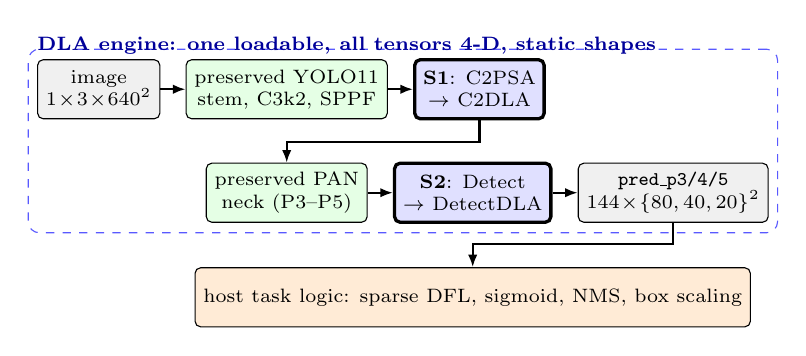
\begin{tikzpicture}[
    node distance=2.6mm and 3.2mm,
    box/.style={draw, rounded corners=2pt, align=center, minimum height=7.5mm,
                inner xsep=3pt, font=\scriptsize},
    kept/.style={box, fill=green!10},
    sub/.style={box, fill=blue!12, very thick},
    io/.style={box, fill=gray!12},
    host/.style={box, fill=orange!16},
    ar/.style={-{Latex[length=1.6mm]}, thick}
]
\node[io] (img) {image\\$1\!\times\!3\!\times\!640^2$};
\node[kept, right=of img] (bb) {preserved YOLO11\\stem, C3k2, SPPF};
\node[sub, right=of bb] (mix)
  {\textbf{S1}: C2PSA\\$\rightarrow$ C2DLA};
\node[kept, below=5.5mm of bb] (neck) {preserved PAN\\neck (P3--P5)};
\node[sub, right=of neck] (head) {\textbf{S2}: Detect\\$\rightarrow$ DetectDLA};
\node[io, right=of head] (maps) {\texttt{pred\_p3/4/5}\\$144\!\times\!\{80,40,20\}^2$};
\node[host, below=5.5mm of head] (post)
  {host task logic: sparse DFL, sigmoid, NMS, box scaling};

\draw[ar] (img) -- (bb);
\draw[ar] (bb) -- (mix);
\draw[ar] (mix.south) -- ++(0,-2.7mm) -| (neck.north);
\draw[ar] (neck) -- (head);
\draw[ar] (head) -- (maps);
\draw[ar] (maps.south) -- ++(0,-2.7mm) -| (post.north);

\node[draw=blue!65, dashed, rounded corners,
      fit=(img)(bb)(mix)(neck)(head)(maps), inner sep=3.2pt] (engine) {};
\node[font=\scriptsize\bfseries, blue!60!black, above=0.4mm of engine.north west,
      anchor=west] {DLA engine: one loadable, all tensors 4-D, static shapes};
\end{tikzpicture}%
}
\caption{Accelerator boundary and the two substitutions. The learned graph inside the
dashed region compiles to one DLA loadable in the evaluated configuration.
Preprocessing, physical-layout conversion, and detection decoding run on the host. S1 removes the
attention matrix multiplications, S2 removes the rank-three decoded output
interface. Green blocks are inherited from the reference model unchanged.}
\label{fig:boundary}
\end{figure}

\subsection{Design Objective and Scope}
Let $G_0$ denote the reference learned graph and $G$ the adapted graph. We
seek a useful detector subject to
\begin{equation}
 \operatorname{Build}_{\mathrm{DLA}}(G;\theta,\mathrm{fallback}=0)
 = E, \qquad N_{\mathrm{GPU}}(E)=0,
 \label{eq:accept}
\end{equation}
where $\theta$ fixes the target, compiler version, precision, shapes, and
I/O formats, $E$ is the serialized engine, and $N_{\mathrm{GPU}}$ counts
GPU-assigned learned layers after optimization. For the evaluated artifact we
also require one DLA loadable. These are deployment criteria, not terms in the
training loss. Accuracy and application performance must be evaluated after
this feasibility gate.

We retain the convolutional stem, C3k2 stages, SPPF module, feature-pyramid
connections, and detection towers of YOLO11n. Two module substitutions define
the adaptation:
\begin{equation}
 \mathrm{C2PSA}\longrightarrow\mathrm{C2DLA},\qquad
 \mathrm{Detect}\longrightarrow\mathrm{DetectDLA}.
 \label{eq:substitutions}
\end{equation}
The first changes a learned computation; the second changes the export
boundary while preserving the ordinary training path. This separation permits
an architecture comparison on the GPU and a placement comparison using the
same adapted graph. It does not make the stock and adapted engine interfaces
identical.

\subsection{C2DLA: Channel Mixing with Local Context}
\label{sec:c2dla}
\begin{figure}[t]
\centering
\resizebox{\columnwidth}{!}{%
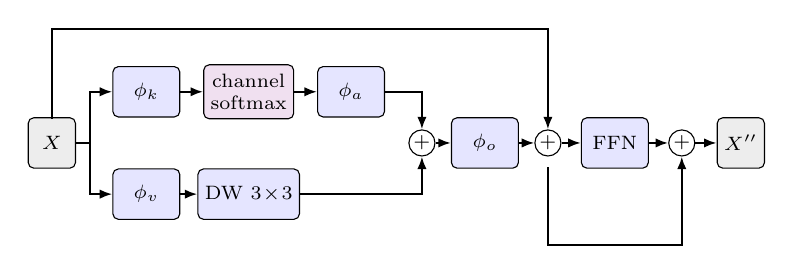
\begin{tikzpicture}[
    op/.style={draw, rounded corners=2pt, align=center, minimum height=6.4mm,
               minimum width=8.5mm, inner xsep=2.5pt, font=\scriptsize},
    conv/.style={op, fill=blue!10},
    act/.style={op, fill=violet!12},
    io/.style={op, fill=gray!14, minimum width=6mm},
    sum/.style={draw, circle, inner sep=0.5pt, font=\scriptsize},
    ar/.style={-{Latex[length=1.6mm]}, thick}
]
\node[io]   at (0.25,-0.65) (b)   {$X$};
\node[conv] at (1.45,0)     (pk)  {$\phi_k$};
\node[act]  at (2.75,0)     (sm)  {channel\\softmax};
\node[conv] at (4.05,0)     (pa)  {$\phi_a$};
\node[conv] at (1.45,-1.30) (pv)  {$\phi_v$};
\node[conv] at (2.75,-1.30) (dw)  {DW $3\!\times\!3$};
\node[sum]  at (4.95,-0.65) (s1)  {$+$};
\node[conv] at (5.75,-0.65) (po)  {$\phi_o$};
\node[sum]  at (6.55,-0.65) (r1)  {$+$};
\node[conv] at (7.40,-0.65) (ffn) {FFN};
\node[sum]  at (8.25,-0.65) (r2)  {$+$};
\node[io]   at (9.00,-0.65) (out) {$X''$};

\draw[ar] (b.east) -- ++(0.18,0) |- (pk.west);
\draw[ar] (b.east) -- ++(0.18,0) |- (pv.west);
\draw[ar] (pk) -- (sm);
\draw[ar] (sm) -- (pa);
\draw[ar] (pv) -- (dw);
\draw[ar] (pa.east) -| (s1.north);
\draw[ar] (dw.east) -| (s1.south);
\draw[ar] (s1) -- (po);
\draw[ar] (po) -- (r1);
\draw[ar] (r1) -- (ffn);
\draw[ar] (ffn) -- (r2);
\draw[ar] (r2) -- (out);
% residual around the mixer, Eq. (8)
\draw[ar] (0.25,-0.34) -- (0.25,0.80) -- (6.55,0.80) -- (r1.north);
% residual around the FFN, Eq. (9)
\draw[ar] (6.55,-0.96) -- (6.55,-1.95) -- (8.25,-1.95) -- (r2.south);
\end{tikzpicture}%
}
\caption{The inner C2DLA block. Channel softmax makes the upper branch
input-dependent at each position; the $3\times3$ depthwise branch supplies local
spatial context. Both residuals, the feed-forward block, and the enclosing
split--process--merge structure are retained. The replacement does not compute
global spatial attention.}
\label{fig:c2dla}
\end{figure}

C2DLA keeps C2PSA's split--process--merge structure. An initial $1\times1$
projection produces two channel groups; one bypasses the inner block and the
other is processed before concatenation and a final projection. If $X$ is the
processed group with $C$ channels, define
\begin{align}
 K &= \phi_k(X), \qquad V=\phi_v(X), \label{eq:kv}\\
 A_{bkhw} &= \frac{\exp K_{bkhw}}{\sum_{j=1}^{d}\exp K_{bjhw}},
 \label{eq:chansoftmax}\\
 Z &= \phi_o\bigl(\phi_a(A)+\psi_{3\times3}(V)\bigr),
 \label{eq:mix}\\
 X' &= X+Z, \label{eq:res1}\\
 X'' &= X'+\operatorname{FFN}(X'). \label{eq:res2}
\end{align}
Here $d=\max(\lfloor C/4\rfloor,8)$; $\phi_k:C\to d$,
$\phi_v:C\to C$, $\phi_a:d\to C$, and $\phi_o:C\to C$ are
$1\times1$ projections. The operator $\psi$ is a $3\times3$ depthwise
convolution. The FFN expands channels from $C$ to $2C$, applies SiLU, and
projects back to $C$. Batch normalization accompanies the relevant convolution
modules and is folded into them for inference; $\phi_a$ is a bias-free
convolution without batch normalization.

For the nano configuration, the enclosing block receives 256 channels, the
processed group has $C=128$, the bottleneck has $d=32$, and one inner block
operates at the $20\times20$ scale. All operations preserve the four-dimensional
batch--channel--height--width representation. Unlike the original attention,
there is no spatial affinity matrix, matrix multiplication, head transpose,
or normalization over image positions.

The softmax output remains input-dependent: changing a pixel's feature vector
changes its channel weights. However, this branch independently transforms
each spatial position, and its projection back to $C$ channels does not provide
global information exchange. The depthwise branch supplies local spatial
context. The substitution therefore changes the hypothesis class and requires
empirical accuracy evaluation; it is not an algebraic equivalence.

The key and value projections are separate convolutions. This avoids introducing
a fused-QKV extraction subgraph in the replacement branch. Static channel
splits elsewhere in the retained network remain present and compile successfully
in the measured configuration. Thus, the implementation does not depend on a
claim that every split or SiLU is unsupported on DLA.

\subsection{DetectDLA: A Static Prediction Boundary}
\label{sec:boundary}
For each pyramid level $\ell\in\{3,4,5\}$, the retained regression and
classification towers produce $R_\ell$ and $S_\ell$. DetectDLA exports
\begin{equation}
 P_\ell=\operatorname{Concat}_{C}(R_\ell,S_\ell)
 \in\mathbb{R}^{B\times(4r+n_c)\times H_\ell\times W_\ell},
 \label{eq:packed}
\end{equation}
with $r=16$ regression bins and $n_c=80$ COCO classes. For batch one and
$640\times640$ images, the outputs are $1\times144\times80\times80$,
$1\times144\times40\times40$, and $1\times144\times20\times20$ at strides
8, 16, and 32. They are named \texttt{pred\_p3}, \texttt{pred\_p4}, and
\texttt{pred\_p5}. Classification values are logits; box channels are
unnormalized distributions, not decoded coordinates.

In export mode, the head stops before flattening, cross-scale concatenation,
DFL expectation, grid decoding, and sigmoid. NMS is also outside the engine.
During training and ordinary PyTorch inference, DetectDLA invokes the inherited
Detect path, retaining its losses and assignment behavior. No direct-regression
or one-to-one head is introduced in this study.

The static maps make the execution boundary explicit. Stock YOLO11n's engine
instead emits a decoded $1\times84\times8400$ tensor. At FP16, the adapted
outputs contain 2,419,200 bytes, compared with 1,411,200 bytes for the stock
output, a factor of 1.714. Consequently, a lower raw-engine latency does not
by itself establish a faster complete detector: the adapted pipeline transfers
more data and performs additional host decoding.

\begin{table}[t]
\caption{The evaluated adaptation. Unchanged denotes retained structure, not
identical trained weights.}
\label{tab:design}\centering\footnotesize
\setlength{\tabcolsep}{3pt}
\begin{tabular}{p{.26\columnwidth}p{.31\columnwidth}p{.32\columnwidth}}
\toprule
Component & YOLO11n & \model \\
\midrule
Stem, C3k2, SPPF, neck & Reference structure & Unchanged \\
Terminal mixer & Spatial self-attention & Channel softmax and local DWConv \\
Box/class towers & Distributional boxes; class logits & Unchanged \\
Training head & Original Detect & Inherited Detect path \\
Export output & One decoded rank-3 tensor & Three raw rank-4 tensors \\
Host detection logic & NMS & DFL, sigmoid, NMS \\
\bottomrule
\end{tabular}
\end{table}

\subsection{Training and Initialization}
The compatible structure permits transfer of shape-matched parameters from a
YOLO11 checkpoint before fine-tuning. The accompanying code also contains an
optional block-aware initializer that gathers compatible key/value projection
channels and copies positional and output projections. The new channel
projection has no direct self-attention counterpart. This optional path and a
staged freeze/unfreeze recipe are implementation capabilities; the retained
checkpoint does not establish that either was used for its training run.

The checkpoint actually evaluated here contains a 500-epoch training history,
with batch size 32, image size 640, seed 0, automatic optimizer selection,
pretrained initialization requested, AMP enabled, and no frozen layers in the
stored training arguments. It contains 2,615,696 unfused parameters. The exact
initialization source and realized optimizer settings must be recovered before
attributing accuracy to a particular transfer strategy.
\missing{P2}{archive the original training command, initialization checkpoint,
optimizer state/log, dataset identity, and independently repeated validation}.

\section{Export and Runtime}
\label{sec:deployment}
\subsection{Exported Graph and Strict Compilation}
The retained ONNX artifact uses opset 20 and a static $1\times3\times640\times640$
input. Inspection finds 89 convolutions, 76 sigmoid and 76 multiplication nodes,
9 splits, 14 additions, 20 concatenations, 3 max-pooling operations, 2 resizes,
and one softmax. There are no MatMul, Gemm, Reshape, Transpose, Div, or Slice
operators. The sigmoid/multiplication pairs represent retained SiLU activations;
operator counts before fusion are not execution-kernel counts.

Compilation targets DLA core 0 in FP16 with GPU fallback disabled and explicit
native I/O formats. Successful compilation is checked against both the verbose
placement report and the optimized-engine inspector. A one-node DLA inspector
result is evidence of a single compiled loadable, not a claim that the original
network contains one operation. The build and profile records remain linked to
the engine name, compiler version, and output bindings.

This audit is configuration-specific. TensorRT's DLA softmax support depends on
the target and shape, and the compiler warns that the selected approximation
can introduce numerical error \cite{nvidia_dla_working}. A source-level
rewrite that compiles on this Orin/TensorRT combination is not sufficient
evidence for another DLA generation, input size, or precision. Build success
also does not validate raw-output decoding.

\subsection{Native Layouts and the Host Boundary}
\label{sec:packing}
The strict build requests \texttt{fp16:dla\_hwc4} input and
\texttt{fp16:chw16} outputs. Its inspector describes a DLA image input format
and sixteen-channel-vectorized outputs. For this three-channel image, the
physical input buffer pads channels to four and uses interleaved pixel storage;
the $640$-pixel row satisfies the documented 64-byte alignment. The buffer
occupies $4\times640\times640\times2=3{,}276{,}800$ bytes. Each output has
144 channels, already divisible by 16, so CHW16 requires no extra channel
padding.

The reference runner converts between these buffers and logical NCHW tensors
on the CPU using tensor views, permutations, materialization, and copies.
Its timed stages include both packing and H2D transfer at the input, and both
D2H transfer and unpacking at the output. They cannot be interpreted as pure
layout-conversion timings. A CUDA stream and device-visible buffers are still
used for execution and transfer even when the learned graph has no GPU layers.

Logical shape is insufficient to allocate or interpret a native binding.
Runtime validation must record format descriptions, vectorized dimensions,
components per element, and context strides, then test the corresponding
packing rules. The retained summary uses a CHW4 shorthand for the input;
we follow the build's requested DLA format and require a runtime record before
treating format names as interchangeable.
\missing{P4}{archive binding formats/strides and raw multi-image timing records}.

\subsection{Confidence-First Host Decoding}
\label{sec:decode}
The host splits each $P_\ell$ into 64 regression channels and 80 class channels.
For confidence threshold $\tau\in(0,1)$, an anchor survives if
\begin{equation}
 \max_c S_{\ell,c}(h,w) > \log\frac{\tau}{1-\tau}.
 \label{eq:threshold}
\end{equation}
This is equivalent in exact arithmetic to applying sigmoid and then the same
maximum-class threshold. Regression decoding is independent of class
confidence, so it can be postponed until after this rejection step. For each
survivor and box side $q\in\{l,t,r,b\}$, the DFL expectation is
\begin{equation}
 \hat d_q=\sum_{j=0}^{r-1}j\,
 \frac{\exp R_{qj}}{\sum_{k=0}^{r-1}\exp R_{qk}}.
 \label{eq:dfl}
\end{equation}
The decoder places cell centers at $(w+0.5,h+0.5)$, forms the four box
coordinates from these distances, scales by the level stride, applies class
sigmoid, and performs class-aware NMS. The final coordinates are mapped back
through the image's letterbox transform.

If $m$ of $N=8400$ anchors survive, dense class scanning remains
$O(Nn_c)$, while the regression softmax/expectation work falls from $O(4rN)$
to $O(4rm)$. This does not reduce raw-output transfer volume. The repeated-image
summary reports $m=13$ at $\tau=0.25$, a favorable case that cannot establish
the candidate distribution on a dataset.

The equivalence argument assumes identical threshold strictness, class
selection, NMS settings, and tie handling. Floating-point behavior near the
threshold, multi-label validation, and NMS ordering require explicit tests.
\missing{P3}{measure raw-output agreement and dense/sparse decoder parity,
including low-confidence dataset validation}.

\section{Experimental Evaluation}
\label{sec:eval}
We ask whether the adaptation (i) enables complete DLA placement, (ii) provides
useful detection accuracy, and (iii) changes engine and application costs.
Evidence is separated by provenance: raw build/timing artifacts support the
placement and engine results; an embedded training history supports the
checkpoint metrics; a consolidated experiment summary provides provisional
application measurements. These sources do not offer equal validation.

\subsection{Platform, Artifacts, and Timing Protocol}
\label{sec:setup}
The device logs identify an NVIDIA Orin, compute capability 8.7, 16 streaming
multiprocessors, and 62,840\,MiB of reported device memory. TensorRT reports
version 10.3.0; strict execution targets DLA core 0. These properties are
recorded directly, but they do not uniquely establish the carrier configuration
or active operating conditions.
\missing{P1}{record exact module/carrier, JetPack/L4T, CUDA, power mode,
clock policy, temperatures, and matching artifact hashes}.

All engine comparisons enable FP16, with batch one and $640\times640$ inputs.
TensorRT may retain FP32 intermediates in GPU/fallback regions; this flag is
not a guarantee that every operation executes in FP16. The strict engine's
external bindings are FP16.
Each configuration has one \texttt{trtexec} launch with a 2\,s warm-up, a 30\,s
timing interval, one inference stream, spin waiting, generated input data, and
transfers enabled. The logged latency is
\begin{equation}
 L_{\mathrm{engine+IO}} = T_{\mathrm{H2D}}+T_{\mathrm{device}}+T_{\mathrm{D2H}}.
 \label{eq:latency}
\end{equation}
It excludes preprocessing, external decode, and NMS. On a DLA engine,
TensorRT's field named ``GPU Compute Time'' measures the device-execution
interval and does not prove GPU computation. Saturated throughput is completed
queries divided by host wall time; overlapping transfer and execution means
it need not equal the reciprocal of median latency.

The four retained timing traces contain 8,651 stock-GPU, 9,519 adapted-GPU,
878 stock-fallback, and 1,119 strict-DLA samples, matching the logged timed
counts. These are within-launch samples, not independent experimental repeats.
Reported P95 values describe those traces; they are not confidence intervals
on performance across launches or boards. Layer profiles were collected in
separate runs and are interpreted separately from transfer-inclusive timing.

\subsection{Fallback-Free Placement}
\label{sec:placement}
Stock YOLO11n fails strict compilation at its attention MatMul. The adapted
artifact compiles successfully; its build report assigns 299 layers to DLA and
reports no layers on the GPU. The optimized inspector represents the learned
graph as exactly one DLA layer with the three raw prediction outputs. Together,
the fallback-disabled build and inspector satisfy Eq.~\eqref{eq:accept} for
the recorded configuration.

The stock model with GPU fallback enabled produces a different result.
Its pre-optimization placement report assigns 317 layers to DLA and 17 to the
GPU. After optimization, the inspector contains four DLA loadables, eleven GPU
compute nodes, twenty-two reformat nodes, and ten no-op/constant nodes.
Figure~\ref{fig:profile} groups the optimized nodes and their measured profile
time. This is a successful heterogeneous deployment, but it does not meet the
complete learned-graph placement objective.

\begin{figure}[t]
\centering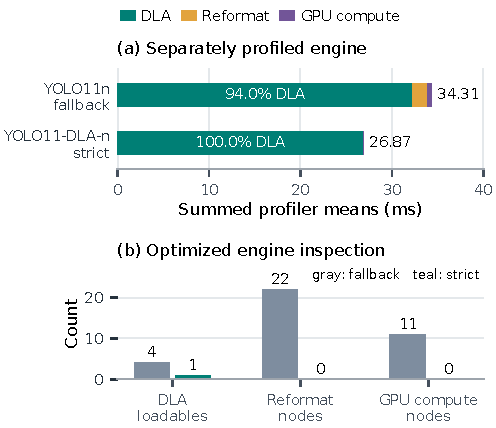
\includegraphics[width=\columnwidth]{figures/fallback_profile.pdf}
\caption{Stock YOLO11n with GPU fallback and the adapted strict-DLA engine.
Node counts come from engine inspection; time shares and summed means come
from separate layer-profile runs. DLA dominates the fallback engine's time
despite four loadables and intervening GPU/reformat work.}
\label{fig:profile}
\end{figure}

The four DLA loadables account for 93.97\% of profiled time, reformat nodes for
4.73\%, and GPU compute nodes for 1.30\%. The device profile totals about
34.312\,ms, including 32.244\,ms in DLA segments. These categories identify
where this compiled engine spends time. They do not isolate the causal cost of
partitioning: the strict graph also changes the attention computation and the
output interface. A matched-graph placement ablation is needed for that claim.

\subsection{Latency and Throughput at the Engine Boundary}
\label{sec:engine}
Table~\ref{tab:engine} reports the complete deployment matrix for YOLO11.
The strict adapted engine achieves 27.515\,ms median engine-plus-transfer
latency versus 34.678\,ms for stock YOLO11n with fallback. This is a 20.7\%
reduction, with throughput increasing from 29.2 to 37.2 queries/s (27.6\%).
Thus, the two graph changes enable complete DLA placement while improving
this engine-boundary comparison.

\begin{table}[t]
\caption{TensorRT FP16, batch one, $640\times640$. Latency includes transfers.
Each measured row is one launch; P95 is a within-launch percentile. Stock
strict DLA failed to build, so it has no timing result.}
\label{tab:engine}\centering\footnotesize
\setlength{\tabcolsep}{3pt}
\begin{tabular}{llrrr}
\toprule
Model & Device & Median & P95 & Rate \\
 & & (ms) & (ms) & (q/s) \\
\midrule
YOLO11n & GPU & 3.740 & 3.753 & 288.3 \\
YOLO11n & DLA+GPU & 34.678 & 34.942 & 29.2 \\
YOLO11n & Strict DLA & \multicolumn{3}{c}{Build rejected} \\
\model & GPU & 3.500 & 3.512 & 317.2 \\
\model & Strict DLA & 27.515 & 27.718 & 37.2 \\
\bottomrule
\end{tabular}
\end{table}

\begin{figure}[t]
\centering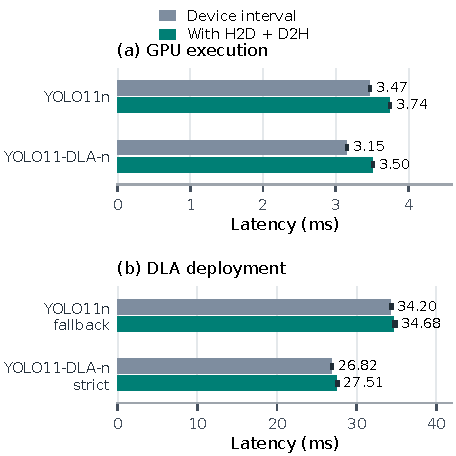
\includegraphics[width=\columnwidth]{figures/latency_comparison.pdf}
\caption{Device-execution and transfer-inclusive latency for the four successful
builds, with different horizontal scales for GPU and DLA panels. Medians and
P95 endpoints are computed from the retained timing traces;
the endpoints represent within-run variation. Device and total quantiles are
computed separately.}
\label{fig:latency}
\end{figure}

Figure~\ref{fig:latency} also exposes the cost of choosing DLA over the GPU.
The adapted model's GPU engine has a 3.500\,ms median, making its strict-DLA
execution 7.86 times slower. Relative to stock YOLO11n on the GPU, the ratio is
7.36. Median strict-DLA device execution is approximately 26.816\,ms; transfers
are a small component of this microbenchmark. This observation applies to the
measured engine and does not imply that its execution time is an unavoidable
lower bound for other compiler configurations or model variants.

The adapted GPU engine is slightly faster than the stock GPU engine, but their
output boundaries differ. Removing in-engine decode and modifying attention
both affect the comparison. We therefore use the adapted GPU row primarily as
a same-model execution control. Neither its engine timing nor the stock-fallback
comparison establishes complete-pipeline superiority.

\subsection{Accuracy Evidence and Training Record}
\label{sec:accuracy}
The retained adapted checkpoint embeds 500 epochs of training validation.
Table~\ref{tab:accuracy} reports its stored final metrics and
Fig.~\ref{fig:training} plots the retained history. The final AP is 37.581,
and AP$_{50}$ is 53.151, on the checkpoint's configured COCO validation task
\cite{lin2014coco}. These are checkpoint-recorded metrics, not a new independent
validation run. Stored validation precision and recall are 65.034\% and 48.557\%.

\begin{table}[t]
\caption{Accuracy provenance. AP is COCO AP averaged over IoU thresholds
0.50:0.05:0.95, in percentage points. Missing values are not inferred from model
names or literature benchmarks.}
\label{tab:accuracy}\centering\footnotesize
\setlength{\tabcolsep}{3pt}
\begin{tabular}{p{.40\columnwidth}ccp{.21\columnwidth}}
\toprule
Model / evaluation & AP & AP$_{50}$ & Evidence \\
\midrule
\model / training validation & 37.581 & 53.151 & Stored epoch 500 \\
YOLO11n / matched PyTorch & \missing{P2}{AP} & \missing{P2}{AP} & Pending \\
\model / independent PyTorch & \missing{P2}{AP} & \missing{P2}{AP} & Pending \\
\model / strict DLA & \missing{P3}{AP} & \missing{P3}{AP} & Pending \\
\bottomrule
\end{tabular}
\end{table}

\begin{figure}[t]
\centering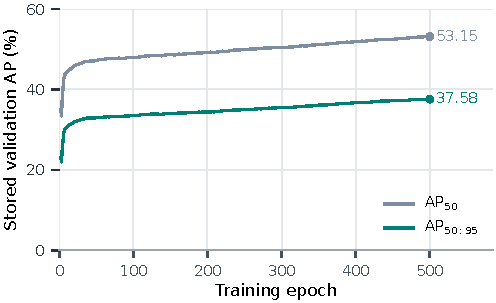
\includegraphics[width=\columnwidth]{figures/training_history.pdf}
\caption{Validation history embedded in the retained \model{} checkpoint.
This is one recorded 500-epoch training run, without repeated-seed uncertainty
or a paired stock-YOLO11n training curve. It is not serialized-engine accuracy.}
\label{fig:training}
\end{figure}

A paired reference evaluation under identical preprocessing and evaluator
settings is absent. Accordingly, no measured accuracy-retention percentage or
accuracy-loss claim is made. The exported ONNX and engines also need a verified
identity chain back to the checkpoint, because filenames do not certify that
they contain the same weights. The remaining numerical test must distinguish
three effects: the changed architecture, export/FP16 arithmetic, and the native
runtime/decoder path.

\subsection{Local Export and Decoder Verification}
\label{sec:parity}
We additionally execute a reproducible CPU check on the retained checkpoint and
ONNX artifact, using one $1\times3\times640\times640$ uniform-random input
with seed 7. External dense decoding of the adapted PyTorch raw maps agrees
with the same model's ordinary decoded output: maximum absolute error is
$1.22\times10^{-4}$, and mean absolute error is $5.45\times10^{-8}$. The
elementwise comparison passes with relative tolerance $10^{-5}$ and absolute
tolerance $10^{-4}$; these tolerances are combined, not separate maximum-error
limits. The output has shape $1\times84\times8400$ before NMS.

ONNX Runtime CPU inference also agrees with the checkpoint's three raw outputs
under relative/absolute tolerances $10^{-4}/10^{-3}$. Maximum absolute errors
are $2.08\times10^{-4}$, $3.07\times10^{-4}$, and $6.87\times10^{-5}$ for
P3, P4, and P5. ONNX structural validation and the output-shape checks pass.
The script records artifact and input hashes plus library versions. These
checks exercise the export interface and dense decoder on one input; they
do not compare against stock YOLO11, certify sparse NMS equivalence, or execute
the serialized DLA engine.

\subsection{Application Measurements: Provisional Evidence}
\label{sec:application}
The experiment summary retains results from a sequential runner with ten warm-up
iterations and 100 timed repetitions of one $960\times1280$ image. It uses
CPU post-processing, confidence 0.25, and NMS IoU 0.45, excluding file reading,
drawing, and writing. The original YOLO11-family per-frame JSON records are not
present in the supplied log directory. Table~\ref{tab:e2e} is therefore
explicitly a transcription of summary-level evidence, pending recollection.

\begin{table}[t]
\caption{Provisional repeated-image pipeline medians in ms, transcribed from the
retained summary. I/O sums the pack/H2D and D2H/unpack stage medians. Medians need not
sum to median total. \missing{P4}{replace with raw multi-image results}.}
\label{tab:e2e}\centering\footnotesize
\setlength{\tabcolsep}{3pt}
\begin{tabular}{lrrrrr}
\toprule
Model / device & Pre & I/O & Engine & Post & Total \\
\midrule
11n / GPU & 4.900 & 2.843 & 8.153 & 3.250 & 19.203 \\
11n / DLA+GPU & 8.617 & 4.002 & 35.198 & 4.866 & 52.782 \\
11-DLA / GPU & 4.572 & 3.848 & 7.560 & 3.717 & 19.831 \\
11-DLA / DLA & 8.946 & 13.992 & 27.788 & 5.711 & 56.497 \\
\bottomrule
\end{tabular}
\end{table}

These preliminary totals reverse the engine-boundary ordering between strict
DLA and stock fallback: 56.497 versus 52.782\,ms. The sum of the strict path's
I/O stage medians is 13.992\,ms, including conversion and transfer; its host
decode is additional work relative to stock YOLO11n's decoded output. Different
preprocessing times for the same image and code also reveal uncontrolled
between-launch conditions. Without raw traces and platform telemetry, those
differences cannot be assigned to CPU clocks, thermals, or accelerator
contention. Summing or subtracting stage medians does not provide an exact
per-frame decomposition.

The summary reports matching classes and displayed confidences for the adapted
GPU and DLA paths, with at most 0.3 pixels difference in displayed box
coordinates on this image. This is a provisional smoke check, not dataset-level
numerical equivalence. No energy measurements or concurrent-task timing results
are present in the supplied evidence.

\section{Validation Gaps and Robotics Experiments}
\label{sec:discussion}
\subsection{Numerical Correctness of the Deployed Detector}
The highest-priority experiment is validation through the exact serialized
strict-DLA engine. A conventional backend that allocates linear buffers from
logical tensor shapes cannot be assumed to support DLA-native formats. The
validator must use format-aware allocation and packing, decode raw outputs with
the same class and coordinate conventions, and preserve the official COCO image
and category mappings. AP, AP$_{50}$, AP$_{75}$, and small/medium/large-object
AP should be reported for stock PyTorch, adapted PyTorch, adapted GPU FP16,
and strict DLA FP16 on the same 5,000 validation images.

Detection validation must retain low-confidence candidates and the evaluator's
multi-label and maximum-detection settings. The confidence-0.25 visual smoke
test is not a suitable AP protocol. Numerical checks should first compare raw
maps and decoded predictions on matched preprocessed inputs, then report
aggregate AP changes. This separates layout errors from the compiler's softmax
approximation and ordinary FP16 rounding.
\missing{P3}{fill strict-engine accuracy, raw-output errors, and decoder parity}.

\subsection{Ablations for the Model and Interface}
The observed compatibility result combines two changes. A controlled ablation
should use stock attention or C2DLA, crossed with decoded or raw output. Stock
attention with raw outputs isolates the attention blocker; C2DLA with decoded
outputs isolates the export boundary. These controls require fresh compiler
records rather than predictions based only on source operators. GPU accuracy
controls remain meaningful even when their strict builds fail.

A second comparison should hold the training schedule fixed while varying
shape-matched initialization, block-aware transfer, and random initialization
of the replacement block. At least three seeds would expose sensitivity to the
new mixer. A convolution-only replacement with comparable capacity would test
whether channel softmax adds accuracy worth its compiler constraints.
\missing{P5}{report build outcome, AP, parameters, and timing for these controls}.
The current single training history cannot isolate those effects or establish
that C2DLA is an optimal replacement.

\subsection{GPU Contention and Robotic Replay}
A strict learned graph does not establish isolation of the whole application.
The CPU, memory controller, power envelope, transfers, and runtime remain shared.
The first experiment should measure a fixed GPU workload alone and beside each
perception placement: stock GPU, adapted GPU, stock fallback, and adapted strict
DLA. For a co-running task with latency quantile $Q_p$, define
\begin{equation}
 S_p=\frac{Q_p(L_{\mathrm{co\text{-}running}})}
             {Q_p(L_{\mathrm{standalone}})}.
 \label{eq:slowdown}
\end{equation}
Report both median and P95 slowdown, perception latency, delivered frame rate,
and deadline misses. Use independent launches in randomized order, retaining
per-frame timestamps and clock/temperature traces. A synthetic CUDA workload
provides a repeatable stress test but does not establish a robotics benefit.

A second experiment should replay a timestamped camera sequence through a ROS~2
perception node \cite{macenski2022ros2}, alongside a specified GPU mapping or
navigation component. Keep image order, frame-release times, queue capacity, and
drop policy fixed across placements. Report acquisition-to-result latency,
queue delay, dropped frames, perception deadline misses, and co-running-task
slowdown. Compute service time alone omits the delay that a controller observes.
\missing{P6}{insert measured contention and robotic-replay results}.

\subsection{Energy at a Matched Delivered Rate}
DLA placement may change power, but longer execution and additional host work
can offset a lower device power level. Energy must therefore be integrated over
the same measured interval as completed frames:
\begin{equation}
 E_{\mathrm{frame}}=\frac{\int_{t_0}^{t_1}P_{\mathrm{board}}(t)\,dt}
 {N_{\mathrm{completed}}}.
 \label{eq:energy}
\end{equation}
Report total board energy and, separately, idle-subtracted energy using an idle
measurement under the same power mode and clock policy. Compare placements at
a common delivered rate that all can sustain, as well as under saturation;
otherwise a lower frame count can obscure the comparison. Record the rail
being sampled, its sampling interval, and alignment with runtime timestamps.
Avoid adding overlapping board and component power rails.
\missing{P7}{insert power, joules/frame, achieved rate, and repeat variability}.

\subsection{Limits of the Present Evidence}
The hardware evidence covers one Orin configuration, TensorRT 10.3, FP16, one
input resolution, and one detector scale. It establishes neither INT8 behavior
nor portability across DLA generations. Generated-input microbenchmarks exclude
content-dependent host decoding; the provisional repeated-image experiment
samples only one scene. No claim of energy savings, global GPU isolation,
hard real-time behavior, or accuracy preservation follows from strict
compilation alone. These limits define what the additional experiments must
resolve rather than changing the compatibility result already observed.

\section{Conclusion}
YOLO11-DLA adapts YOLO11 through a channel-softmax/local-convolution replacement
and a static raw-output interface. The nano instance compiles into one
fallback-free DLA loadable on the measured Orin/TensorRT stack, where stock
YOLO11n fails strict compilation. Its 27.515\,ms median engine-plus-transfer
latency is 20.7\% lower than stock YOLO11n with GPU fallback, while remaining
7.86 times slower than its own GPU engine. The retained training record reports
37.581 AP; deployed-engine accuracy is still pending. The contribution is a
concrete DLA-compatible YOLO11 implementation and an auditable characterization
of its execution boundary. Dataset validation and concurrent robotics/energy
experiments will determine when this placement is useful within a complete
robot system.

\section*{Acknowledgment}
OpenAI Codex (GPT-6) assisted with drafting and revision of all manuscript
sections, source-code and log inspection, and generation of the plotting code,
figures, and tables. Numerical results were drawn from the supplied artifacts;
missing experiments are marked explicitly. \missing{P8}{authors to verify all
claims, references, figures, and final AI disclosure before submission}.

\bibliographystyle{IEEEtran}
\bibliography{references}
\end{document}
